\section*{Random Number Generators}
\subsection*{Lehmers Random}
\begin{algorithm}[H]
\SetAlgoLined
\KwIn{a, c, m, x}
\KwOut{Random number between 0 and 1}
\SetKwFunction{lehmersinit}{lehmers\_init}
\SetKwFunction{lehmersrand}{lehmers\_rand}
\SetKwProg{Fn}{Function}{:}{end}
\Fn{\lehmersrand{a=None, c=None, m=None, x=None}}{
    global lehmers\_vars\;
    \uIf{$Variables\ Not\ Initialized$}{
        \uIf{a == None or c == None or m == None or x == None}{
            \lehmersinit{$7^5, 0, 2^{31} - 1, 1.0$}\;
        }
        \Else{
            \lehmersinit{$a, c, m, x$}\;
        }
    }
    \Else{
        \tcp{Generate a random number using Lehmer's formula}
        $x = (a\cdot x +c) \mod{m}$;
    }
    \KwRet $x/m$\;
}
\caption{Lehmer's Random Number Generator}
\label{alg:lehmersrand}
\end{algorithm}
\subsubsection*{BNumMet Examples}
\paragraph{Example 1}{
\begin{lstlisting}[language=Python]
from BNumMet.Random import lehmers_rand
for i in range(10):
    print(lehmers_rand())

>> Lehmers Random Number Generator Initialized with default values
	a=16807
	c=0
	m=2147483647
	x=1.0
    7.826369259425611e-06
    0.13153778814316625
    0.7556053221950332
    0.4586501319234493
    0.5327672374121692
    0.21895918632809036
    0.04704461621448613
    0.678864716868319
    0.6792964058366122
    0.9346928959408276
\end{lstlisting}
}
\paragraph{Example 2: Predictability of Lehmer's Random Number Generator}{
\begin{lstlisting}[language=Python]
from BNumMet.Random import lehmers_rand, clear_lehmers_vars
clear_lehmers_vars()
arr = [1]
for i in range(10):
    aux = lehmers_rand(a=2**16 + 3, m=2**31, c=0, x=arr[-1])
    if len(arr) >= 3:
        lehmerFormula = (6 * arr[-1] - 9 * arr[-2]) % 1  # Test Xn = (6Xn-1 - 9Xn-2)
        print(f"Lehmer's = {aux}\nPredicted = {lehmerFormula}\n")
    arr.append(aux)

>>  Lehmer's = 0.0008239871822297573
    Predicted = 0.0008239871822297573
    
    Lehmer's = 0.003295936156064272
    Predicted = 0.003295936156064272
    
    Lehmer's = 0.012359732296317816
    Predicted = 0.012359732296317816
    
    Lehmer's = 0.04449496837332845
    Predicted = 0.04449496837332845
    
    Lehmer's = 0.15573221957311034
    Predicted = 0.15573221957311034
    
    Lehmer's = 0.533938602078706
    Predicted = 0.533938602078706
    
    Lehmer's = 0.8020416363142431
    Predicted = 0.8020416363142431
    
    Lehmer's = 0.006802399177104235
    Predicted = 0.006802399177104235
\end{lstlisting}
}
\paragraph{Example 3: Visual failure}{
\begin{lstlisting}[language=Python]
from BNumMet.Random import lehmers_rand, clear_lehmers_vars
clear_lehmers_vars()
fail2 = (
    lambda: float(
        (int(lehmers_rand(a=65539, c=0, m=2**31, x=123) * (2**31)) >> 23) & 0xFF
    )
    / 255
)
fail = [(fail2(), fail2()) for i in range(100000)]
plt.scatter(*zip(*fail), s=1, c="black")
plt.show()
\end{lstlisting}
\begin{figure}[H]
    \centering
    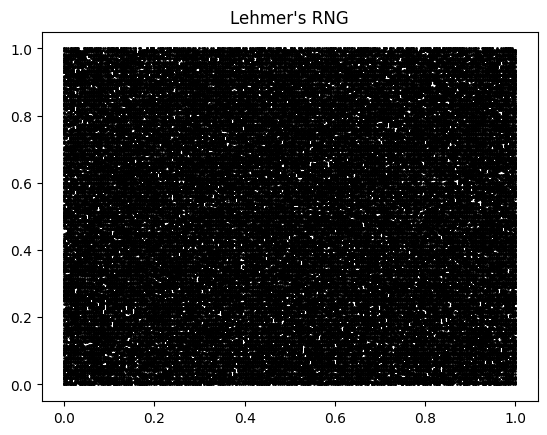
\includegraphics{Include/Images/Thesis/Documentation/Randomness/Lehmers Rand Example 3.png}
    \caption{Lehmers Rand Example 3}
    \label{fig:Lehmers Rand Example 3}
\end{figure}
}


\subsection*{Marsaglia's Random Generator}
The algorithm is based of \cite{10.1214/aoap/1177005878} the original paper where Gearge Marsaglia and Arif Zaman discussed it.

\begin{algorithm}[H]
\SetAlgoLined
 \SetKwInOut{Input}{Input}
 \SetKwInOut{Output}{Output}
 \SetKwProg{Fn}{Function}{:}{end}
 
 \Input{base, lag\_r, lag\_s, carry, seed\_tuple}
 \Output{The generated random number}
 \Fn{marsaglia\_rand($base, lag\_r, lag\_s, carry, seed\_tuple$)}{
 global marsaglia\_vars\;
 \eIf{(global dictionary marsagliaVars is NOT initialized)}{
   \eIf{(Some inputs are NONE)}{
     marsaglia\_init($2^{31} - 1, 19, 7, 1, (1, 1)$)\;
   }{
     marsaglia\_init(base, lag\_r, lag\_s, carry, seed\_tuple)\;
   }
 }{
 }
 $x_{new} = x_0 - x_{lag_r-lag_s} - carry$\;
 \eIf{$x_{new}$ < 0}{
   $x_{new} += base$\;
   $carry = 1$\;
 }{
   $carry = 0$\;
 }
 $\overrightarrow{x} = [x(1:),\ x_{new}]$\\
 \Return $x_{new} / base$\;
 }
 \caption{Marsaglia Random Number Generator Algorithm}
\end{algorithm}

\subsubsection*{BNumMet Examples}
\paragraph{Example 1}{
\begin{lstlisting}[language=Python]
from BNumMet.Random import marsaglia_rand, clear_marsaglia_vars
clear_marsaglia_vars()
for i in range(10):
    print(marsaglia_rand(base=41, lag_r=2, lag_s=1, carry=0, seed_tuple=(0, 1)))

>>  0.975609756097561
    0.024390243902439025
    0.926829268292683
    0.0975609756097561
    0.8048780487804879
    0.2926829268292683
    0.4878048780487805
    0.8048780487804879
    0.6585365853658537
    0.12195121951219512
\end{lstlisting}
}
\paragraph{Example 2}{
\begin{lstlisting}[language=Python]
from BNumMet.Random import marsaglia_rand, clear_marsaglia_vars
clear_marsaglia_vars()
fail = [
    (
        marsaglia_rand(base=100, lag_r=2, lag_s=1, carry=0, seed_tuple=(0, 1)),
        marsaglia_rand(base=100, lag_r=2, lag_s=1, carry=0, seed_tuple=(0, 1)),
    )
    for i in range(100000)
]
plt.scatter(*zip(*fail), s=1, c="black")
\end{lstlisting}
\begin{figure}[H]
    \centering
    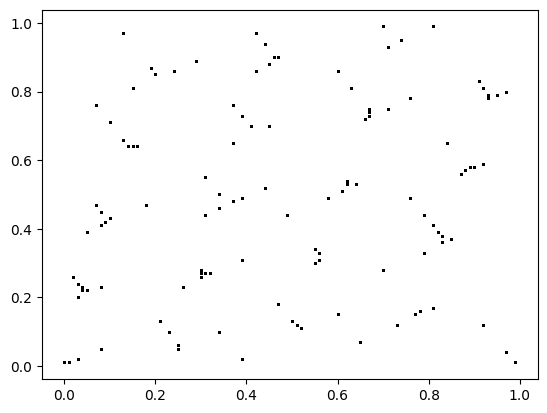
\includegraphics{Include/Images/Thesis/Documentation/Randomness/Marsaglia Rand Example 2.png}
    \caption{Marsaglia Rand Example 2}
    \label{fig:Marsaglia Rand Example 2}
\end{figure}
}
\paragraph{Example 3}{
\begin{lstlisting}[language=Python]
from BNumMet.Random import marsaglia_rand, clear_marsaglia_vars
clear_marsaglia_vars()
fail = [
    (
        marsaglia_rand(base=41, lag_r=2, lag_s=1, carry=0, seed_tuple=(0, 1)),
        marsaglia_rand(base=41, lag_r=2, lag_s=1, carry=0, seed_tuple=(0, 1)),
    )
    for i in range(100000)
]
plt.scatter(*zip(*fail), s=1, c="black")
\end{lstlisting}
\begin{figure}[H]
    \centering
    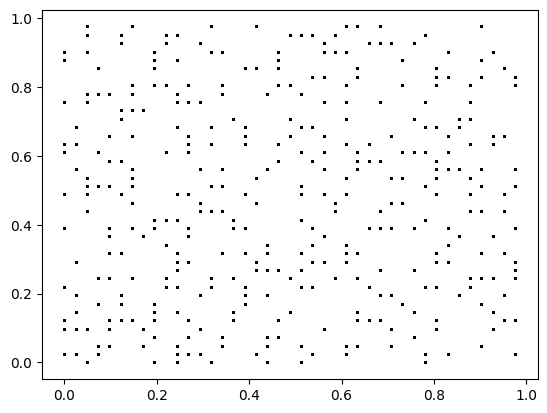
\includegraphics{Include/Images/Thesis/Documentation/Randomness/Marsaglia Rand Example 3.png}
    \caption{Marsaglia Rand Example 3}
    \label{fig:Marsaglia Rand Example 3}
\end{figure}
}

\subsection*{Mersenne Twister Random Generator}
The algorithm was based of \cite{10.5555/148286} which is an implementation of the Mersnne Twister in the programming language of C. The implementation has been tested using the NIST Random test suite \cite{smid2010statistical}, more on this on the Analaysis of Solutions section*

\begin{algorithm}[H]
\SetAlgoLined
\SetKwFunction{sgenrand}{sgenrand}
\SetKwFunction{genrand}{genrand}
\SetKwProg{Fn}{Function}{:}{}
\Fn{\genrand{seed: int = None}}{
\tcp{global variables}
global mt, mti, mag01\\

\If{mtVars is not initialized}{
    \If{seed is None}{
        seed = 4357
    }
    \sgenrand{seed}
}
    
    mag01 = [0x0, A]\\
    \If{mti $\geq$ N}{
        kk = 0\;
        y = None\;
        \While{kk $<$ N - M}{
            y = (mt[kk] \&\& UPPER\_MASK) $||$ (mt[kk + 1] \&\& LOWER\_MASK)\;
            mt[kk] = mt[kk + M] $\oplus$ (y $>>$ 1) $\oplus$ mag01[y \& 0x1]\;
            kk += 1\;
        }
        \While{kk $<$ N - 1}{
            y = (mt[kk] \& UPPER\_MASK) $|$ (mt[kk + 1] \& LOWER\_MASK)\;
            mt[kk] = mt[kk + (M - N)] $\oplus$ (y $>>$ 1) $\oplus$ mag01[y \&\& 0x1]\;
            kk += 1\;
        }
        y = (mt[N - 1] \&\& UPPER\_MASK) $||$ (mt[0] \&\& LOWER\_MASK)\;
        mt[N - 1] = mt[M - 1] $\oplus$ (y $>>$ 1) $\oplus$ mag01[y \& 0x1]\;
        mti = 0\;
    }
    
    y = mt[mti]\;
    mti += 1\;
    
    \tcp{Tempering}
    y $\oplus$= TEMPERING\_SHIFT\_U(y)\;
    y $\oplus$= (TEMPERING\_SHIFT\_S(y) \& TEMPERING\_MASK\_B)\;
    y $\oplus$= (TEMPERING\_SHIFT\_T(y) \& TEMPERING\_MASK\_C)\;
    y $\oplus$= TEMPERING\_SHIFT\_L(y)\;
    
    \KwRet y / 0xFFFFFFFF\;
}
\caption{Mersenne Twister Random Number Generator}
\end{algorithm}
\remark{
\begin{enumerate}
    \item $\oplus$ Operator stands for a bitwise XOR
    \item $\&\&$ Operator stands for a bitwise AND
    \item $||$ Operator stands for a bitwise OR
\end{enumerate}
}

\subsubsection*{BNumMet Examples}
\paragraph{Example 1}{
\begin{lstlisting}[language=Python]
from BNumMet.Random import clear_mt_vars,genrand
clear_mt_vars()
for i in range(10):
    print(genrand())

>>  Initialized the global dictionary mtVars with seed 4357
    0.8173300600185361
    0.9990608997175147
    0.5103543725587322
    0.13153290984489324
    0.03541634837990076
    0.9924695345089932
    0.6257087035630151
    0.06259194576707482
    0.4107105111262553
    0.13477367491805314
\end{lstlisting}
}
\paragraph{Example 2}{
\begin{lstlisting}[language=Python]
from BNumMet.Random import clear_mt_vars,genrand
clear_mt_vars()
toPlot = [(genrand(),genrand()) for i in range(100000)]
plt.scatter(*zip(*toPlot), s=1, c="black")
\end{lstlisting}
\begin{figure}[H]
    \centering
    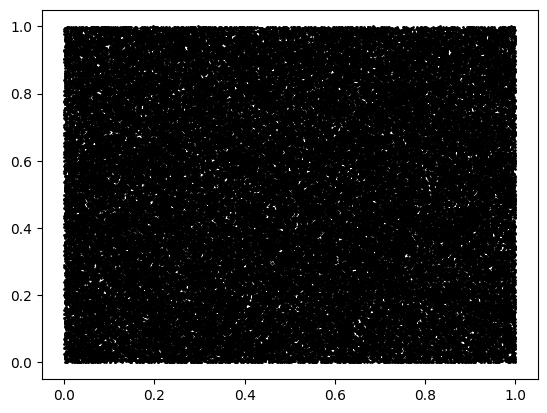
\includegraphics{Include/Images/Thesis/Documentation/Randomness/MersenneTwister Rand Example 2.png}
    \caption{Mersenne Twister Rand Example 2}
    \label{fig:Mersenne Twister Rand Example 2}
\end{figure}
}